\begin{figure}[h]
  \centering
  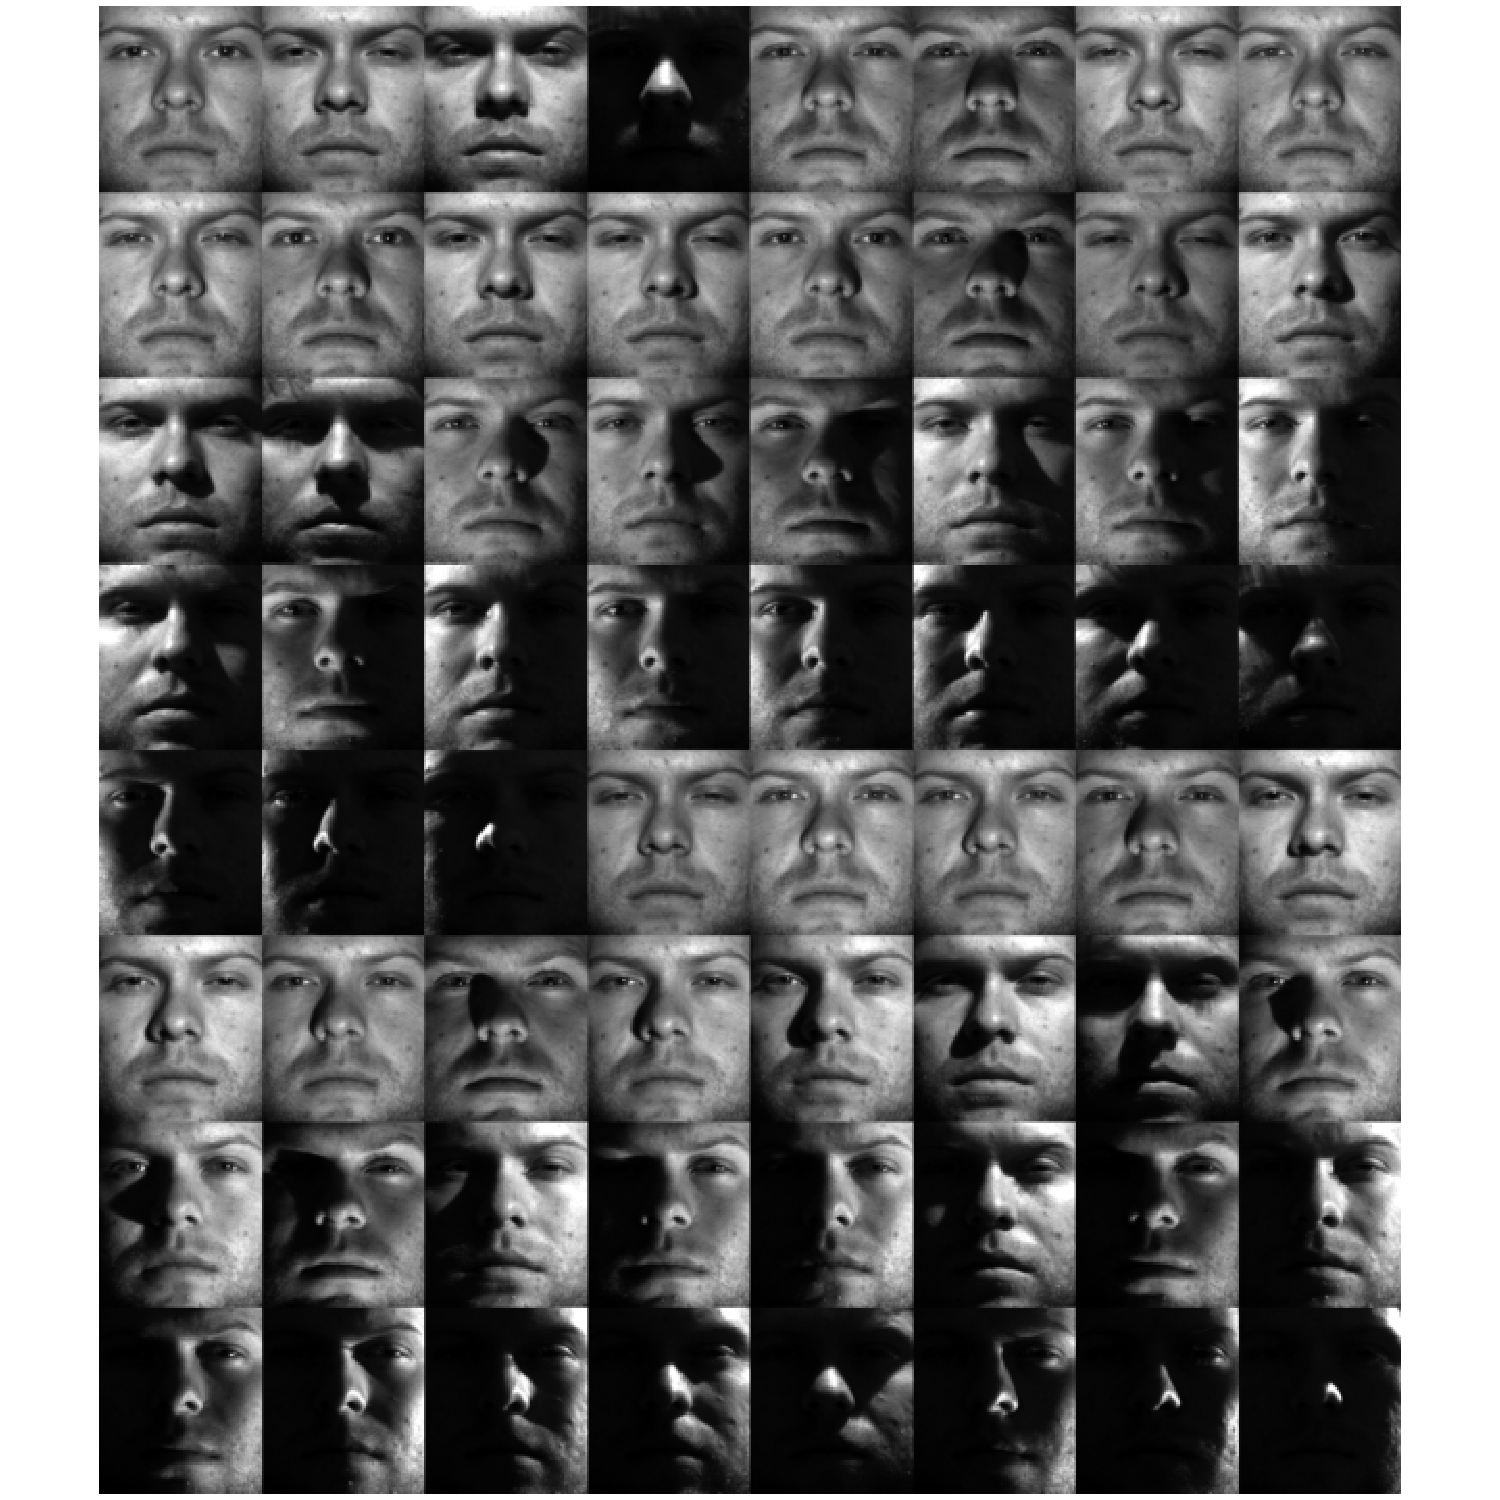
\includegraphics[width=\columnwidth]{P01.pdf}
  \caption{All images of person 1 under 64 different lighting conditions generated with the geodesic dome}
  \label{P01}
\end{figure}

\begin{figure}[htbp]
  \centering
  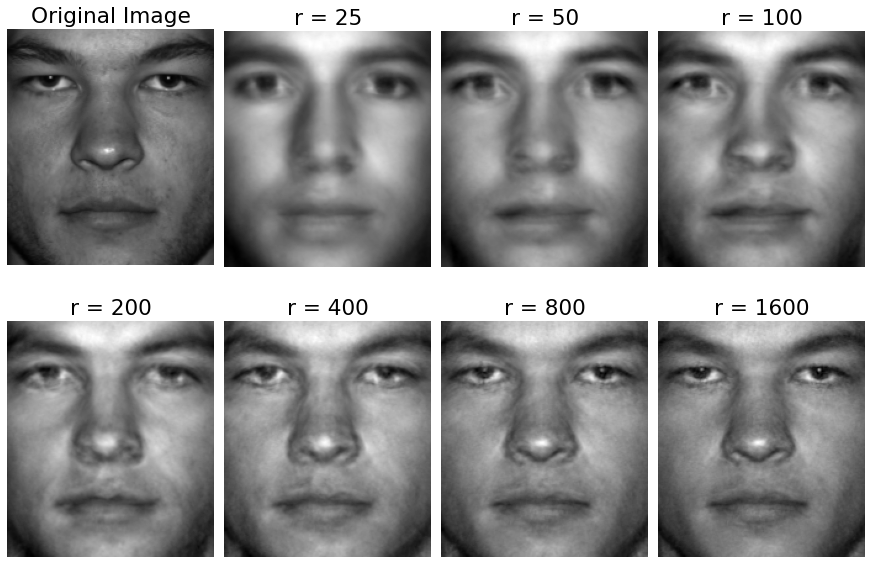
\includegraphics[width=\columnwidth]{reconstruction.png}
  \caption{Approximate representation of sample image using eigenfaces basic of various order $r$. Test image is not in training set. the approximation is relatively poor for $r\leq200$, although for $r>400$ it converges to a passable representation of the test image.}
  \label{appendix:reconstruction}
\end{figure}

\begin{figure}[htbp]
  \centering
  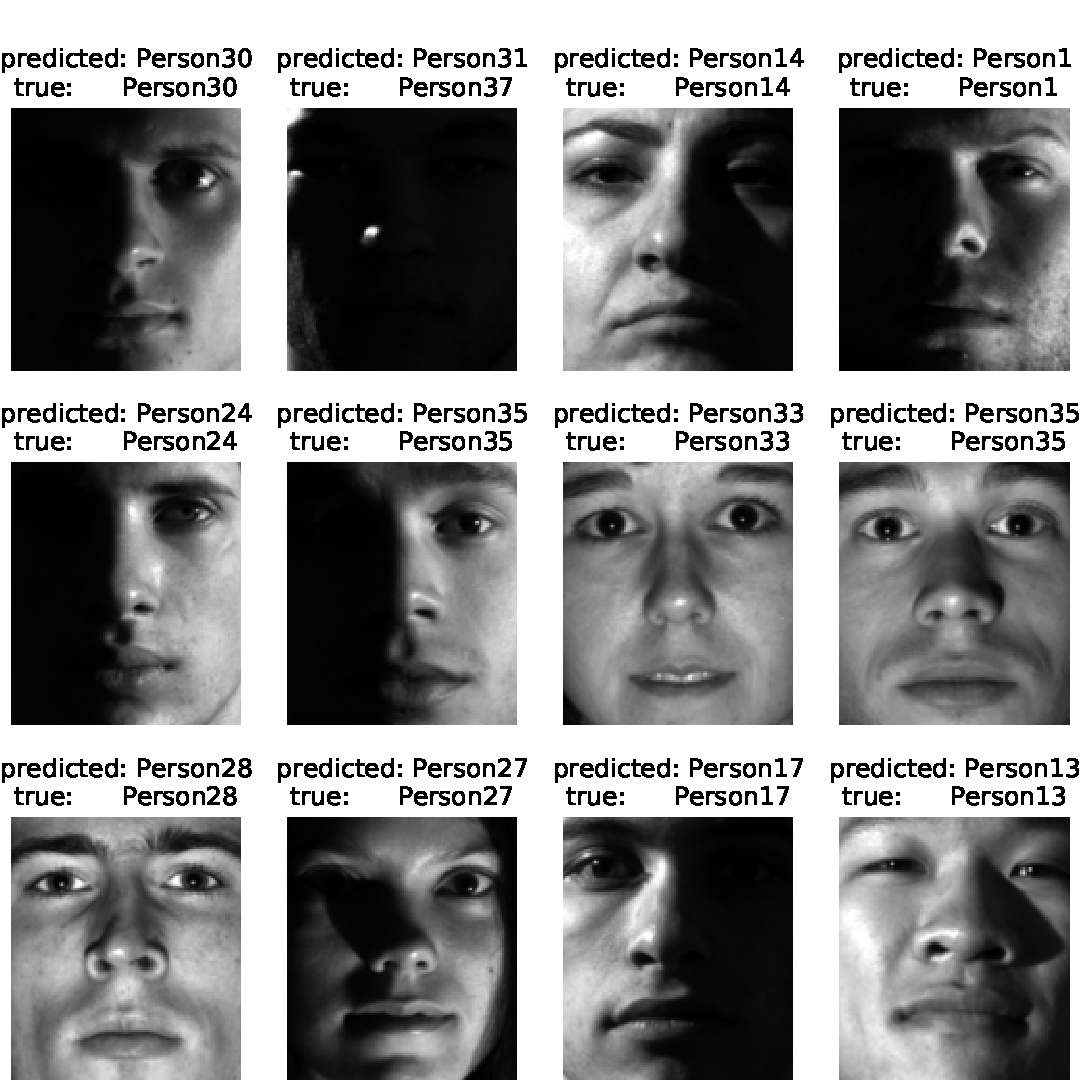
\includegraphics[width=\columnwidth]{PCAgallery.pdf}
  \caption{Qualtitative evaluation of PCA+SVM predictions on first 12 samples of the test set}
  \label{appendix:PCAgallery}
\end{figure}

\begin{figure}[htbp]
  \centering
  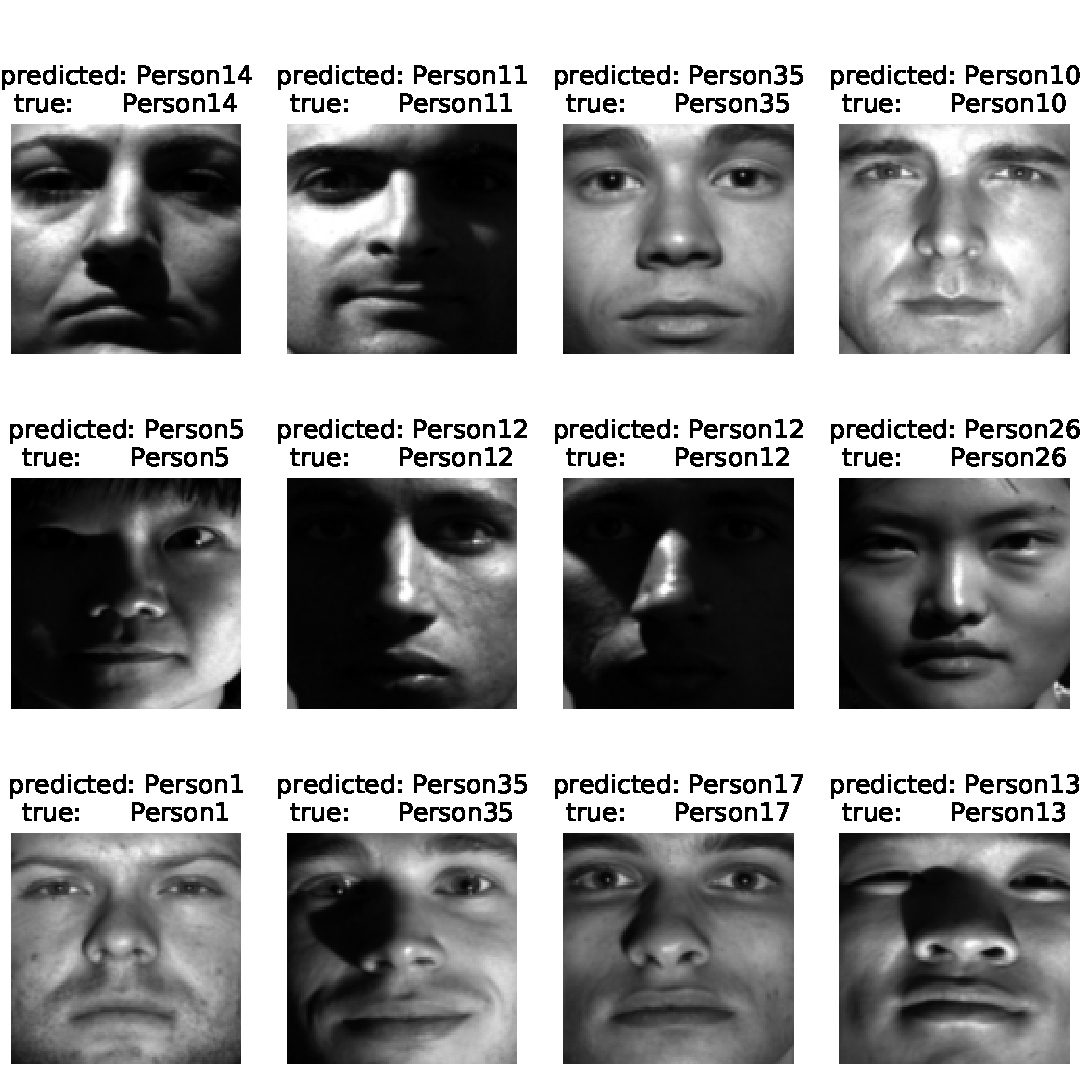
\includegraphics[width=\columnwidth]{EncoderGallery.pdf}
  \caption{Qualitative evaluation of Autoencoder+Softmax predictions on first 12 samples of the test set}
  \label{appendix:Encodergallery}
\end{figure}

\begin{figure}[p]
  \centering
  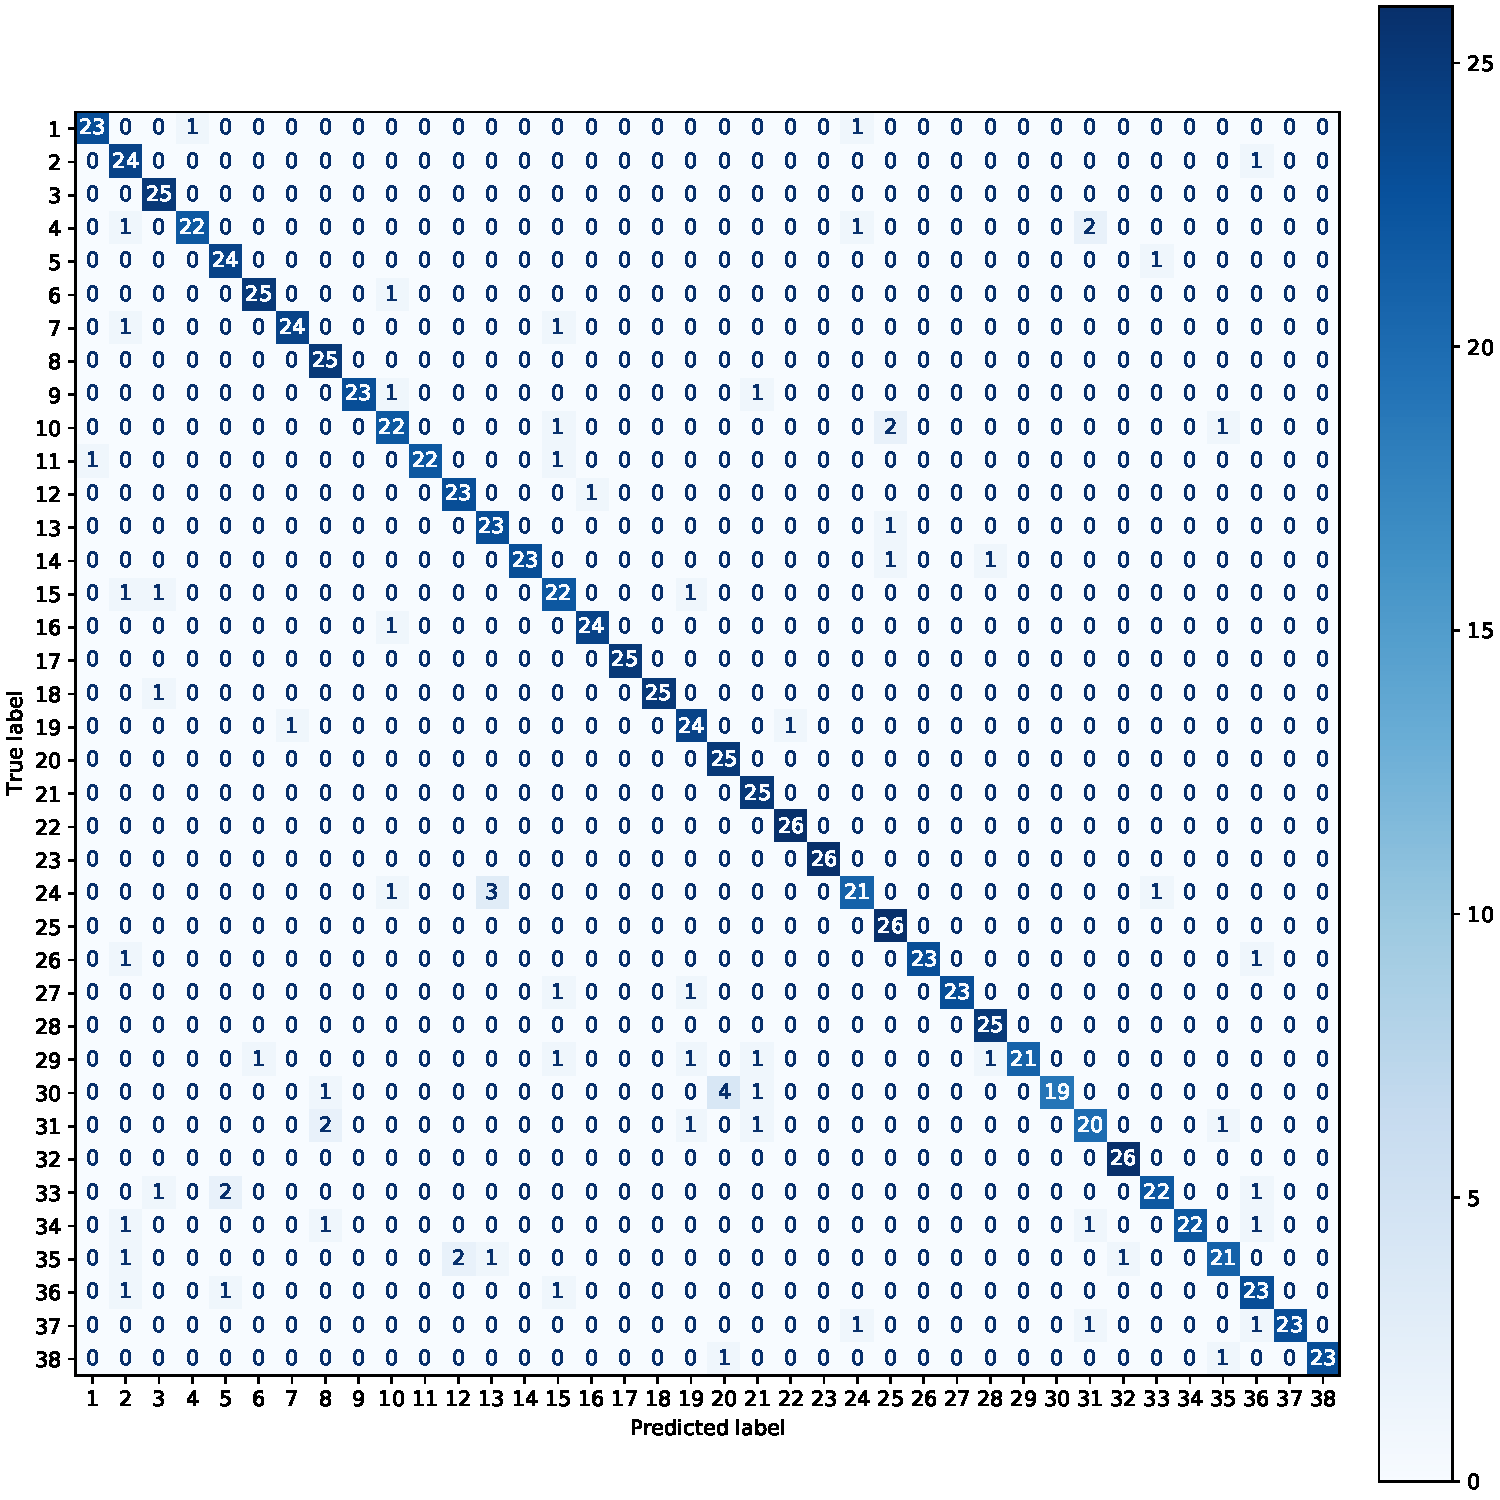
\includegraphics[width=\paperwidth]{PCAconfusion.pdf}
  \caption{The confusion matrix in face recognition at application of PCA}
  \label{appendix:PCAconfusion}
\end{figure}
